\documentclass{article}
\usepackage[latin1]{inputenc}    
\usepackage[T1]{fontenc}
\usepackage[french]{babel}
\usepackage{graphicx}
\newcommand\tab[1][1cm]{\hspace*{#1}}
\usepackage{geometry}
\geometry{hmargin=3.45cm,vmargin=3cm}
\usepackage{color}
\definecolor{myblue}{rgb}{0.15, 0.15, 0.8}

\begin{document}

\newpage
\title{Cahier des spécifications\\Sujet 10 : Réseau de Neurones}
\author{Thibaut \bsc{Pepin}\\Soumia \bsc{Rezgui}\\Isaac \bsc{Szulek}\\Severine \bsc{Selaquet}\\Anthony \bsc{Montigne}\\Arezki \bsc{Slimani}}
\maketitle

\newpage

\small{\tableofcontents}

\newpage

\section{Structures de Données}
	\subsection{Réseau de neurones}
	Pour le choix de notre structure de données nous avons rapidement adopté la représentation d'un réseau de neurone comme un ensemble de couches et non comme un ensemble de neurone individuel. Chaque Couche devait donc contenir l'ensemble des activation, des biais et des poids des neurones de cette couches sous la forme de vecteurs pour les activations et les biais et sous forme de matrice pour les poids, nous les avons integré dans une structure couche comme tableau a une ou deux dimensions car les calculs a effectuer necessite d'acceder aux éléments sans ordre particulier.
	
	Afin de stocker l'ensemble des couches constituant le réseau de neurone, nous avons opté pour une liste doublement chainé, en effet, les deux algorithme necessitant d'acceder aux contenues des couches vont propager des information de la premiere couche a la derniere couche pour l'algorithme de propagation et de la derniere couches a la premiere couche pour l'algorithme de rétro-propagation, d'ou le double chainage.
	
	Afin de regrouper les informations générales d'un réseau de neurone, nous avons créer une petite structure contenant toutes sortes d'informations comme la date de création.
	
	Un réseau de neurone est donc constitué d'une structure d'information ainsi que d'un pointeur sur la premiere couche et d'un autre pointeur sur la derniere couche.

	\begin{flushleft}
	
		struct COUCHE	//structure représentant une couche (ensemble de neurones) dans un réseau de neurone\\
		\{\\
			\tab \textcolor{myblue}{\textbf{float*}} A;	//tableau représentant le vecteur des activation des neurone d'une couche.Possède autant d'élements que de neurone présent dans la couche\\
			\tab \textcolor{myblue}{\textbf{float*}} B;	//tableau représentant le vecteur des biais des neurone d'une couche. De meme taille que A\\
			\tab \textcolor{myblue}{\textbf{float**}} W;	//tableau a deux dimensions représentant la matrice des poids entre les neurones de la couches précedente et les neurones de cette couche. Ce tableau est donc de taille (taille de la couche actuelle x taille de la couche précedente) et est composé d'élement $w_{ij}$ ou j est le numéro du neurone de la couches précedente et i le numéro du neurone de la couche actuelle.\\
			\tab \textcolor{myblue}{\textbf{int}} taille;	//Indique le nombre de neurones présent dans cette couche\\
			\tab \textcolor{myblue}{\textbf{float}} DELTA;      //tableau représentant le vecteur des modifications a apporter aux biais de cette couches lors de la rétro-propagation des neurone d'une couche.De meme taille que A\\
			\tab \textcolor{myblue}{\textbf{float**}} DELTA\_M; //tableau a deux dimensions représentant la matrice des modifications a apporter aux poids de cette couches lors de la rétro-propagation des neurone d'une couche. De meme taille que W\\
			\medbreak
			\tab \textcolor{myblue}{\textbf{struct COUCHE*}} prec;	//pointeur sur la couche précédente.\\
			\tab \textcolor{myblue}{\textbf{struct COUCHE*}} suiv;	//pointeur sur la couche suivante.\\
		\};\\
		\bigbreak
		typedef struct COUCHE COUCHE;\\
		typedef COUCHE* Liste\_couche;\\
		\bigbreak
		struct INFO\_RN	//structure représentant les différentes informations caractérisant un réseau de neurones.\\
		\{\\
			\tab \textcolor{myblue}{\textbf{char**}} etiquettes;	//tableau de chaine de caractère comprenant la signification des neurones de sortie.\\
			\tab \textcolor{myblue}{\textbf{char*}} nom;	//nom donné au réseau de neurones.\\
			\tab \textcolor{myblue}{\textbf{char*}} date;	//date de création du réseau de neurones.\\
			\tab \textcolor{myblue}{\textbf{int}} reussite;	//nombre de fois ou le réseau de neurone a obtnenue la réponse attendue lors de l'apprentissage.\\
			\tab \textcolor{myblue}{\textbf{int}} echec;	//nombre de fois ou le réseau de neurone n'a pas obtnenue la réponse attendue lors de l'apprentissage.\\
		\};\\
		\bigbreak
		typedef struct INFO\_RN INFO\_RN;\\
		\bigbreak
		struct RN	//structure représentant le réseau de neurones, contenant l'ensemble des couches et les informations du réseau de neurones.\\
		\{\\
			\tab \textcolor{myblue}{\textbf{INFO\_RN}} info;	//les informations du réseau de neurones.\\
			\tab \textcolor{myblue}{\textbf{Liste\_couche}} couche\_deb;	//pointeur sur la 1ere couche du RN.\\
			\tab \textcolor{myblue}{\textbf{Liste\_couche}} couche\_fin;    //pointeur sur la derniere couche du RN.\\
		\};\\
		\bigbreak
		typedef struct RN RN;
		
	\end{flushleft}
	
	\subsection{Image}
	Afin de représenter une image, nous avons opté pour un tableau a une dimension de pixel afin de se rapprocher de la structure des vecteurs d'activations. Chaque pixel étant une structure contenant la quantité de rouge, de vert et de bleu présent dans un nombre entre 0 et 255 d'ou le type char qui convient parfaitement pour des valeur dans cet intervalle.
	\begin{flushleft}
		typedef struct Pixel\\
			\{\\
				\tab \textcolor{myblue}{\textbf{unsigned char}} r,g,b;\\
			\} Pixel;
		\bigbreak
		typedef struct Image\\
			\{\\
				\tab \textcolor{myblue}{\textbf{int}} w,h;\\
				\tab \textcolor{myblue}{\textbf{Pixel*}} dat;\\
			\} Image;
	\end{flushleft}
	
	\subsection{Apprentissage}
	Le couple d'information sortie attendue et donnée d'entrée étant nécessaire lors de l'apprentissage, nous les avons regroupé dans une petite structure.
	\begin{flushleft}
		typedef struct Apprentissage\\
			\{\\
				\tab \textcolor{myblue}{\textbf{Image*}} image;\\
				\tab \textcolor{myblue}{\textbf{char*}} etiquette;\\
			\} App;
	\end{flushleft}
	
	\newpage
	
	
	
	
	
	
\section{Signatures des Fonctions}
	\subsection{Gestionnaires d'apprentissage}
			\subsubsection{\textcolor{myblue}{\textbf{void}} BackProp(\textcolor{myblue}{\textbf{RN*}}, \textcolor{myblue}{\textbf{Image*}} ,\textcolor{myblue}{\textbf{char*}}, \textcolor{myblue}{\textbf{float}})}
				Backprop va effectuer l'algorithme de propagation-inverse puis va modifier les poids et les biais du réseau de neurones passé en paramètre. Pour cela il est nécessaire d'avoir le couple donnée d'entrée et sortie attendue présent ici sous la forme Image* et char*, on effectuera donc la propagation sur l'image et on comparera l'étiquette de sortie avec le char* qui est l'étiquette attendue.
				
			\subsubsection{\textcolor{myblue}{\textbf{void}} SigmoidePrimeZ(\textcolor{myblue}{\textbf{float*}} in, \textcolor{myblue}{\textbf{float**}} out, \textcolor{myblue}{\textbf{int}} taille)}
			SigmoidePrimeZ va récupérer les éléments stockés dans le premier tableau contenant 'taille' éléments puis effectuer l'opération $x*(1-x)$ sur chaque éléments avant de les écrire dans les deuxième tableau passé en paramètre. Cette opération n'est pas la dérivée de la fonction sigmoide, il s'agit d'une petite optimisation qui nous permet de trouver le même résultat plus rapidement. En effet lors de la propagation inverse il nous est necessaire d'effectuer l'opération : \\$\sigma'(z) = \sigma(z)*(1-\sigma(z))$\\ ou z vient de : \\$a^L = \sigma(w^L*a^{L-1}+b^L) = \sigma(z^L)$\\ or z n'est pas stocké dans notre structure et on peut de toute facon simplifier par :\\$\sigma'(z)=a*(1-a)$\\ d'ou cette fonction.\\
			Le deuxième tableau est a deux dimension car DELTA\_M est disponible au moment ou cette opération est effectué, on va donc l'utiliser plutôt que de créer un autre tableau pour stocker le résultat.
			
			\subsubsection{\textcolor{myblue}{\textbf{void}} MultiplicationMatricielleTransposeeTM(\textcolor{myblue}{\textbf{float**}},  \textcolor{myblue}{\textbf{float*}},  \textcolor{myblue}{\textbf{float*}},  \textcolor{myblue}{\textbf{int}},  \textcolor{myblue}{\textbf{int}})\\
			\textcolor{myblue}{\textbf{void}} MultiplicationMatricielleTransposeeMT(\textcolor{myblue}{\textbf{float*}},  \textcolor{myblue}{\textbf{float*}},  \textcolor{myblue}{\textbf{float**}},  \textcolor{myblue}{\textbf{int}},  \textcolor{myblue}{\textbf{int}})}
				Lors de la retro-propagation certaines matrice doivent être transposées, ce qui est pénible a effectuer. Cependant, ces matrices transposées sont toujours multipliée par une autre matrice ce qui nous donne deux cas possible : \\$A^T*B$ ou $B*A^T$\\MultiplicationMatricielleTransposeeTM et MultiplicationMatricielleTransposeeMT représentent ces deux cas mais ne transposent pas de matrice, elle effectue un produit matricielle ou les matrice ne sont pas lu dans le sens conventionnel du produit matriciel afin d'obtenir le même résultat.
				
			\subsubsection{\textcolor{myblue}{\textbf{void}} Hadamard(\textcolor{myblue}{\textbf{float**}},  \textcolor{myblue}{\textbf{float*}},  \textcolor{myblue}{\textbf{float*}},  \textcolor{myblue}{\textbf{int}})}
				Hadamard effectue le produit vectoriel de Hadamard sur les deux premier tableau pour stocker le résultat dans le troisième tableau. Tous ces tableau étant de la même taille, celle ci est passé en paramètre.
				
			\subsubsection{\textcolor{myblue}{\textbf{void}} fct\_cout(\textcolor{myblue}{\textbf{RN}}, \textcolor{myblue}{\textbf{char*}})}
			 fct\_cout va calculer l'erreur entre le résultat obtenue lors de la propagation et le résultat attendu, soit le char*, pour chacun des neurones de la derniere couche du réseau de neurones puis va stocker le résultat dans le tableau DELTA de la derniere couche du réseau.
			
			\subsubsection{\textcolor{myblue}{\textbf{void}} ModifPoids(\textcolor{myblue}{\textbf{float**}},  \textcolor{myblue}{\textbf{float**}},  \textcolor{myblue}{\textbf{int}},  \textcolor{myblue}{\textbf{int}},  \textcolor{myblue}{\textbf{int}} eta)\\
			\textcolor{myblue}{\textbf{void}} ModifBiais(\textcolor{myblue}{\textbf{float*}},  \textcolor{myblue}{\textbf{float*}},  \textcolor{myblue}{\textbf{int}},  \textcolor{myblue}{\textbf{int}} eta)}
			ModifPoids et ModifBiais vont modifier le premier tableau passé en paramètre en lui soustrayant le deuxieme tableau multiplié par la vitesse d'apprentissage 'eta', les autres paramètre sont les tailles des tableaux
		
		
		
	\subsection{Gestionnaire d'entrées sorties}
		\subsubsection{\textcolor{myblue}{\textbf{Image*}} ChargerBmp(\textcolor{myblue}{\textbf{const char*}} fichier,  \textcolor{myblue}{\textbf{int}},  \textcolor{myblue}{\textbf{int}})\\
		\textcolor{myblue}{\textbf{Image*}} ChargerMnist(\textcolor{myblue}{\textbf{const char*}} fichier,  \textcolor{myblue}{\textbf{int}},  \textcolor{myblue}{\textbf{int}})}
		ChargerBmp et ChargerMnist vont lire a l'emplacement donné en paramètre et renvoyer le contenue du fichier sous forme de la structure Image si celui ci contient une image au format bmp non compressé ou au même format que celui utilisé par la base de données MNIST. Le fichier est ensuite supprimé ou partiellement effacé. Les deux entiers correspondent a la largeur et la hauteur maximal de l'image accepté par le réseau de neurone définie par l'utilisateur.
		
		\subsubsection{\textcolor{myblue}{\textbf{int}} Sauver(\textcolor{myblue}{\textbf{Image*}},\textcolor{myblue}{\textbf{const char*}} fichier)}
		Sauver va enregistrer l'image passé en paramètre a l'emplacement lui aussi passé en paramètre au format bmp.
		
		\subsubsection{\textcolor{myblue}{\textbf{Image*}} NouvelleImage(\textcolor{myblue}{\textbf{int}} w,\textcolor{myblue}{\textbf{int}} h)}
		NouvelleImage alloue la mémoire nécessaire pour stocker une image dont la taille est passé en paramètre dans une structure Image puis renvoi l'addresse de l'image créé.
		
		\subsubsection{\textcolor{myblue}{\textbf{Image*}} CopieImage(\textcolor{myblue}{\textbf{Image*}})}
		CopieImage crée une copie de l'image passée en paramètre puis renvoi son addresse.
		
		\subsubsection{\textcolor{myblue}{\textbf{void}} SetPixel(\textcolor{myblue}{\textbf{Image*}},\textcolor{myblue}{\textbf{int}} i,\textcolor{myblue}{\textbf{int}} j,\textcolor{myblue}{\textbf{Pixel}} p)}
			SetPixel modifie le pixel aux coordonnées i*j de l'image passée en paramètre afin de correspondre au pixel p.
		
		\subsubsection{\textcolor{myblue}{\textbf{Pixel}} GetPixel(\textcolor{myblue}{\textbf{Image*}},\textcolor{myblue}{\textbf{int}} i,\textcolor{myblue}{\textbf{int}} j)}
		GetPixel renvoi le pixel aux coordonnées i*j de l'image passée en paramètre.
		
		\subsubsection{\textcolor{myblue}{\textbf{void}} DelImage(\textcolor{myblue}{\textbf{Image*}})}
		DelImage libere la mémoire d'une variable de type Image.
		
		\subsubsection{\textcolor{myblue}{\textbf{char*}} ChargerEtiquetteMNIST(\textcolor{myblue}{\textbf{const char*}} fichier)}
		ChargerEtiquetteMNIST va récupérer la dernière étiquette présente dans le fichier passé en paramètre puis va supprimer celle ci du fichier ou supprimer le fichier si celui ci ne contient plus aucune étiquettes.
		
		\subsubsection{\textcolor{myblue}{\textbf{App*}} ChargementCoupleAttIn(\textcolor{myblue}{\textbf{char*}} repertoire, \textcolor{myblue}{\textbf{int}}, \textcolor{myblue}{\textbf{int}})}
		ChargementCoupleAttIn va rechercher dans le répertoire le premier couple donnée d'entrée et étiquette présent tout en supprimant tout fichier au mauvais format ou non reconnu. Les deux entiers correspondent a la largeur et la hauteur maximal de l'image accepté par le réseau de neurone définie par l'utilisateur.
		
		\subsubsection{\textcolor{myblue}{\textbf{INFO\_RN*}} ChargerInfo()}
		ChargerInfo récupère les structures INFO\_RN de tous les réseaux de neurones enrigistré dans le repertoire ../sav/ et le retourne sous la forme de tableau.
		
		\subsubsection{\textcolor{myblue}{\textbf{RN*}} ChargerRN(\textcolor{myblue}{\textbf{INFO\_RN}} info)}
		ChargerRN initialise et remplie un réseau de neurone dont les informations sont à l'emplacement passé en paramètre avant de renvoyé l'addresse de celui-ci.
		
		\subsubsection{\textcolor{myblue}{\textbf{void}} SaveRN(\textcolor{myblue}{\textbf{RN}})}
		SaveRN va créer ou modifier tous les fichiers nécessaires afin de sauvegarder le réseau de neurone passé en paramètre.
		
	
	\subsection{Gestionnaire du réseau de neurones}
		\subsubsection{\textcolor{myblue}{\textbf{RN*}} initialisation(\textcolor{myblue}{\textbf{INFO\_RN}})}
		Initialise un nouveau réseau de neurones à partir des informations renseignées par l'utilisateur présent dans la structure INFO\_RN passé en paramètre.
		
		\subsubsection{\textcolor{myblue}{\textbf{void}} AjoutCoucheFin(\textcolor{myblue}{\textbf{RN}}, \textcolor{myblue}{\textbf{int}})}
		Ajoute une nouvelle couche a la liste doublement chaînée représentant le réseau de neurone. L'entier passé en paramètre est le nombre de neurone de cette couche.
		
		\subsubsection{\textcolor{myblue}{\textbf{void}} AjoutPremiereCouche(\textcolor{myblue}{\textbf{RN}}, \textcolor{myblue}{\textbf{int}})}
		Ajoute la premiere couche de la liste doublement chaînée représentant le réseau de neurone. L'entier passé en paramètre est le nombre de neurone de cette couche.
		
		\subsubsection{\textcolor{myblue}{\textbf{void}} Propagation(\textcolor{myblue}{\textbf{Image*}}, \textcolor{myblue}{\textbf{RN}})}
		Propagation va récupérer l'image passée en paramètre et va l'enregistrer dans le tableau des activations de la première couche du réseau de neurones. Afin de propager ces informations jusqu'a la dernière couche, la formule suivante va être appliquée sur chacune des couches :\\ $A^j = \sigma(W^j*A^{j-1}+B^j)$\\
		avec j le numéro de la couche.
		
		\subsubsection{\textcolor{myblue}{\textbf{void}} Remplissage(\textcolor{myblue}{\textbf{RN}})}
		Attribution de valeurs aléatoires aux biais et aux poids synaptiques du reseau de neurones passé en argument.
		
		\subsubsection{\textcolor{myblue}{\textbf{char**}} Reconnaissance(\textcolor{myblue}{\textbf{RN}})}
		Retourne les étiquettes des 3 neurones de la dernière couche du réseau possédant les activation les plus élevées sous la forme d'un tableau trié par activation décroissante.
		
		\subsubsection{\textcolor{myblue}{\textbf{void}} MultiplicationMatriceVecteur(\textcolor{myblue}{\textbf{float**}},  \textcolor{myblue}{\textbf{float*}},  \textcolor{myblue}{\textbf{float*}},  \textcolor{myblue}{\textbf{int}},  \textcolor{myblue}{\textbf{int}})}
		Effectue la multiplication de la matrice et du vecteur passés avec en paramètres puis enregistre le résultat dans le troisième tableau. Les deux entiers sont les taille de la matrice et du vecteur.
		
		\subsubsection{\textcolor{myblue}{\textbf{void}} AdditionVecteurVecteur(\textcolor{myblue}{\textbf{float*}},  \textcolor{myblue}{\textbf{float*}},  \textcolor{myblue}{\textbf{float*}},  \textcolor{myblue}{\textbf{int}})}
		Effectue l'addition des deux vecteur passés en paramètre avec en paramètres  puis enregistre le résultat dans le troisième tableau. L'entiers est la taille des deux vecteur.
		
		\subsubsection{\textcolor{myblue}{\textbf{void}} SigmoideV(\textcolor{myblue}{\textbf{float*}},  \textcolor{myblue}{\textbf{float*}},  \textcolor{myblue}{\textbf{int}})}
		SigmoideV applique la fonction sigmoide sur chacun des éléments du premier tableau passé en paramètre puis enregistre le résultat dans le second tableau, l'entier étant la taille de ces tableaux
		
		\subsubsection{\textcolor{myblue}{\textbf{float}} Sigmoide(\textcolor{myblue}{\textbf{float}} x)}
		Sigmoide calcule la sigmoide du nombre passé en paramètre, soit : \\
		$\sigma(x) = \frac{1}{1+e^{-x}}$
	\newpage

\section{circulation d'informations entre les differents modules de l'application}
	\subsection{organigramme et flux d'information}
		%illegal unit of mesure à verifier
		\begin{center} 

			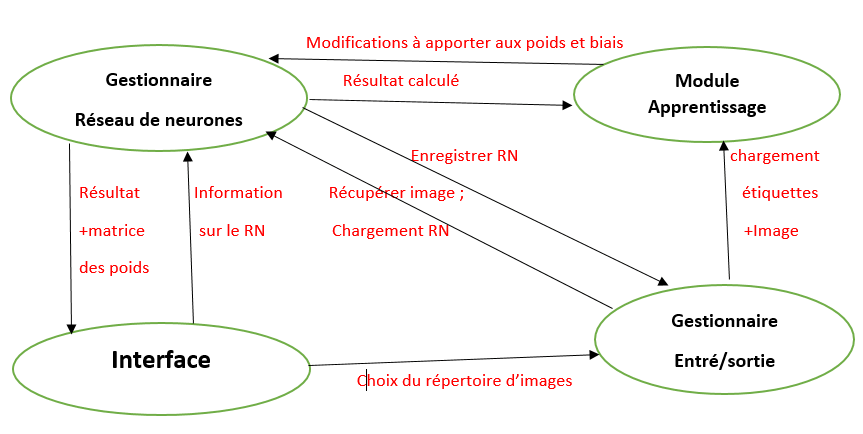
\includegraphics[height=244, width=300]{pic-min.PNG}

		\end{center}	
	\subsection{explication}
		
	Dans l'interface l'utilisateur a la possibilité de choisir un réseau de neurones parmi d'autres déjà crées.pour cela l'information sera transmise au gestionnaire Réseau de neurones afin qu'il puisse charger un réseau de neurones via la fonction chargerRN.
Il peut egalement créer un nouveau réseau de neurones ,dans ce cas-là il devra entrer les données nécessaires pour sa création (couches d'entrées, couches cachées ,neurones de sortie ainsi que les étiquèttes et le format du fichier) ces informations-là seront récupérées par le gestionnaire Réseau de neurones sous forme de structure appelée RN , pour l'utiliser par la suite dans la partie traitement où ce qu'on a appelé propagation, qui dans cette partie ,le réseau de neurones devra récupérer une image du gestionnaire entrée/sortie à travers la structure Image, calculer le résultat et l'envoyer à nouveau à l'interface,ainsi que la matrice des poids pour que l'utilisateur visualise au mieux les opérations qui s'effectuent derrière.Le résultat calculé par le gestionnaire des réseaux de neurones sera récupéré sous forme de fonction propagation par le module Apprentissage pour pouvoir l'utiliser dans la retro-propagation,qui va également récupérer les etiquettes ainsi que l'image du gestionnaire Entrée/sortie via la fonction coupleImageEtiquette qui seront utile pour l'apprentissage.le module Apprentissage recuperera aussi le top 3 des neurones de sortie via la fonction reconnaissance du gestionnaire Reseau de neurones afin qu'on puisse calculer le nombre de reussite et d'echec en comparant la sortie obtenue avec celle attendue.
Par la suite les modifications à apporter aux poids et aux biais seront récupérés par le gestionnaire Réseau de neurones afin de les appliquer.Le Réseau de neurones sera par la suite enregistrer dans le gestionnaire Entrée/Sortie à travers la fonction void SaveRN.
		
		
\end{document}
